% Carleton University SCE 4th Year Project thesis style
% University of Ottawa MSc thesis style -- modifications to the report style
% modification of suthesis style of Stanford University
% Example of use:
\documentclass[12pt]{report}
\usepackage{setspace}
\doublespacing
\usepackage[margin=2.5cm]{geometry}
\usepackage{amsmath,amssymb,amsthm}
\usepackage{graphicx}
%Forces figures to appear within a section, if more specific placement is needed go to:
% http://tex.stackexchange.com/questions/279/how-do-i-ensure-that-figures-appear-in-the-section-theyre-associated-with
\usepackage[section]{placeins}
\usepackage{SCE4YPTemplate}
\usepackage[nottoc,numbib]{tocbibind}
\usepackage{url}
\usepackage[
    backend=bibtex,
    natbib=true,
    style=numeric,
    sorting=none
]{biblatex}
\usepackage[scientific-notation=true, binary-units=true]{siunitx}
\sisetup{per-mode=fraction}%
\sisetup{scientific-notation=false}%

\makeatletter
\def\blx@maxline{77}
\makeatother

\bibliography{report}

\begin{document}
\title{SYSC4907 Project: \\ Sensor-Based Access Control System}
\author{
    Craig Shorrocks,
    Jessica Morris,
    Richard Perryman
}

\copyrightfalse % do not produce a separate copyright page
            % otherwise use \copyrighttrue
%    \figurespagefalse % do not produce a separate figures page
%    \tablespagefalse  % do not produce a separate tables page

% Here you insert the stuff that comes before the preface
% Each preface section is contained in a \prefacesection and starts on a
% new page.  These are numbered using Roman numerals.
% If there are no such pages, do not remove the \beforepreface command
% since it creates the title page.
\beforepreface

%=================================================================================

\prefacesection{Abstract}
    This report tells you all you need to know about something.

%=================================================================================

\prefacesection{Acknowledgements}
    (To be fleshed out more after the first draft)
    We would like to thank:
    \begin{itemize}
    \item Our supervisors, professors Shikharesh Majumdar and Chung-Horng Lung
    \item Jenna Noseworthy and Madeline Ibrahim from the SCE office
    \item Jennifer Wolters (from the Capstone Design fund)
    \item Nagui Mikhail, for soldering lock the hardware
    \item Michel and Normand Leroux, for their construction work on the demo unit for the poster fair
    \end{itemize}

%=================================================================================

% For some reason, these seem to require that you run latex twice?

\prefaceTOC   % to print the Table of Contents
\listoffigures   % to print the List of Figures
\listoftables   % to print the List of Tables

%=================================================================================
                    
\prefacesection{List of Abbreviations}
    
\begin{tabular}[t]{l@{\hspace*{2cm}}l}
    AID & Application IDentifier \\
    APDU & Application Protocol Data Unit \\
    API & Application Programming Interface \\
    HMAC & Keyed-Hash Message Authentication Code \\
	HTML & Hypertext Markup Language \\
	HTTP & Hypertext Transfer Protocol \\
    I2C & Inter-Integrated Circuit \\
    IO & Input/Output \\
    JSON & JavaScript Object Notation \\
    MVC & Model-View-Controller \\
    NFC & Near Field Communication \\
    RFC & Request for Comments \\
    SBACS & Sensor-Based Access Control System \\
\end{tabular}

%=================================================================================

\endpreface
    
%=================================================================================

\chapter{Introduction} \label{introduction}

Give an introduction to your project.  This might include:
\begin{itemize}
  \item Motivation for your project
  \item Problem you are trying to solve
  \item Scope of your project
  \item Organization of your report
\end{itemize}
You should tune this appropriately for what best suits your project.


%=================================================================================

\chapter{The Engineering Project} \label{the-engineering-project}

%=================================================================================

\section{Health and Safety} \label{health-and-safety}

The main health and safety concern for this project was ensuring the safe preparation of circuits for the hardware 
component. The change of bodily harm due to electric shock was possible, as the highest-risk component of the project 
drew $\SI{650}{\milli\ampere}$ of current at 12V direct current. Since $\SI{650}{\milli\ampere}$ is above the 
$\SI{500}{\milli\ampere}$ threshold for possible heart fibrillation~\autocite{CURRENTDANGER}, the following standards
were enforced to mitigate safety risks when handling the electrical components:
\begin{itemize}
    \item The workspace and components were kept dry at all times
    \item Participants ensured they were sufficiently grounded before handling components
    \item Ground pins were connected first, to ensure any charged components would discharge
    \item Components' wiring was not altered while the system was powered on
\end{itemize}
% J - ask if health and safety for construction of the demo unit is necessary here
% (it probably is)

%=================================================================================

\section{Engineering Professionalism} \label{engineering-professionalism}

\begin{itemize}
    \item Teammates were respectful towards one another
    \item Referencing other peoples' works
    \item Acknowledging help from others
    \item Considered diverse viewpoints in developing the project
    \item Considered the ethical ramifications of handling personal information and other secure data
\end{itemize}

%=================================================================================

\section{Project Management} \label{project-management}

This project was sufficiently complicated, that we decided that project management was a necessary tool to facilitate 
the success of the project. We used Github to manage various issues and tasks, as well as for a central 
version-controlled repository. We held weekly meetings to follow the Agile development methodology, doing one-week 
sprints. In these meetings, we demonstrated to each other and our supervisors our progress during the sprint. In our 
project proposal, we planned a timeline that we used to gauge our overall progress. When we fell behind on our planned 
timeline, we isolated areas of work that needed to be accelerated to get back on track. Responsibilities for the 
project were divided evenly among the three team members to balance the work load, and effectively make use of each 
member's time and specialisations. To facilitate system integration, we held informal meetings where we collaborated on 
our work.

(n.b. we will include the Gantt chart from the proposal here)

%=================================================================================

\section{Individual Contributions} \label{individual-contributions}

This section will summarise the contributions each team member made to the project, and to this report.

%---------------------------------------------------------------------------------

\subsection{Project Contributions} \label{project-contributions}

Jessica's contributions:
\begin{itemize}
\item Designed lock circuit, lock control software, and authentication modules
\item Implemented lock circuit, lock control software, and authentication modules
\item Collaborated on the design of the NFC protocol
\end{itemize}

Richard's contributions:
\begin{itemize}
\item Designed the Android application
\item Implemented Android application
\item Collaborated on the design of the NFC protocol
\item Collaborated on HMAC design and implementation
\end{itemize}

Craig's contributions:
\begin{itemize}
\item Designed web server and database
\item Implemented web server and database
\item Collaborated on HMAC design and implementation
\end{itemize}

As a group, we collaborated on system integration, and integration testing.

%---------------------------------------------------------------------------------

\subsection{Report Contributions} \label{report-contributions}

Jessica's contributions:
\begin{itemize}
\item Section 3.4
\item Section 5.4
\item Section 6.2
\end{itemize}

Richard's contributions:
\begin{itemize}
\item Section 5.1, 5.2, 5.3
\item Section 6.1
\end{itemize}

Craig's contributions:
\begin{itemize}
\item Section 5.5
\item Section 6.3
\end{itemize}

All members collaborated on sections 2 and 4.

%=================================================================================

% Consider adding Node, Android? Maybe others?
\chapter{Technical Background} \label{technical-background}

%=================================================================================

\section{NFC} \label{nfc}

%=================================================================================

\section{Cloud Computing} \label{cloud-computing}

%=================================================================================

%---------------------------------------------------------------------------------

\subsection{AWS} \label{aws}

%=================================================================================

\section{Security} \label{security}

%=================================================================================

\section{Single-Board Computers and Microcontrollers} \label{single-board-computers-and-microcontrollers}

A single-board computer, or SOC, incorporates all of the elements necessary for a functional 
computer on a single circuit board: a microprocessor, memory, IO, and other functions. Single-board microcontrollers
(SOMs) have the same intent, to incorporate all of the elements needed to support a microcontroller onto a single
circuit board. The main distinction between SOCs and SOMs is the same as that between computers and microcontrollers.
A microcontroller is designed specifically for one  purpose, such as powering an alarm clock. Whereas, a
computer is a general-purpose computing device, and has more memory, a stronger CPU, and other improved hardware 
features to support the more intense computing needs of a user. As such, it does not require a significant amount of memory, processing 
power, or electricity to perform its task.

%---------------------------------------------------------------------------------

\subsection{Raspberry Pi} \label{raspberry-pi}

The Raspberry Pi is a credit-card-sized, single-board computer developed by the Raspberry Pi Foundation. In its initial 
design, it was intended to be a learning tool to introduce computer science to students at the pre-university  
level. However, its reasonable price gave it increased appeal among hobby electronics enthusiasts, and it is now often 
used for robotics projects, media streaming, IoT projects, and more. Today, the Raspberry Pi has sold over ten million 
units [CITATION], with models ranging from the 5 USD Raspberry Pi Zero, to the 35 USD Raspberry Pi 3 Model B.
% One more paragraph here

%---------------------------------------------------------------------------------

\subsection{Arduino} \label{arduino}



%=================================================================================

\chapter{Business Use Cases} \label{business-use-cases}

Design for our system began with considering use cases that could be handled by our system. This way, we could be sure
to only design features that would prove useful to some potential users, while also making sure that we don't miss any
features that are necessary. These use cases would also provide benefit to demonstrating our system, in that stepping
through a sample use case would show the value of the system to people without them requiring a strong technical
background.

We primarily focused on the four use cases that follow. These were outlined in our initial proposal and have remained
largely unchanged since then. They draw inspiration from situations that we either encountered ourselves or found
through common knowledge and research. Online shopping seemed like a ripe market for technology like the SBACS, and
mail delivery seemed that it followed a fairly similar system. Long term storage facilities also seemed as though they
would benefit from abstracting away the idea of keys. Once we had considered these use cases, we found that several of
the problems that they shared could be solved by a company which provided SBACS as a service. The following subsections
describe these use cases in more detail and provide use-case diagrams summarising them.

%=================================================================================

\section{Online Order Secure Pickup} \label{online-order-secure-pickup}

With online shopping becoming more popular [], the hassle of being physically present to shop in stores 
could be eliminated by allowing customers to make an order and payment online, then pick up their products at the store 
using a SBACS-secured storage container. After a customer's order has been confirmed by the store to be packed 
and ready for pick-up, a store employee could create a link between their customer and the storage container that holds
that user's purchases. When the customer arrives at the store to pick up their items, 
they can gain access to the storage container assigned to them by using the authentication methods that they had
previously provided as the components of their identity. Once the customer has provided these authentication units
correctly, the link between their identity and the storage container is broken. This way, the user will not be able to
inappropriately access the storage container again, and a new link could be made for a different customer. Figure~\ref
{fig:online-order-secure-pickup-use-case} shows a use-case diagram summarising this.

% Todo: add table of actors and system responses

\begin{figure}
    \includegraphics[width=\textwidth]{Diagrams/Use-Case-Diagrams/online-order-secure-pickup-use-case-diagram}
    \caption{Online Order Secure Pickup Use Case Diagram}
    \label{fig:online-order-secure-pickup-use-case}
\end{figure}

A strong advantage of this system over existing ones, such as Walmart's Grab \& Go, is that it creates a digital 
fingerprint using a combination of authentication methods supported by the SBACS, which is more difficult to 
break via brute force than a 6-digit PIN []. In addition, with the entire process of shopping being 
expedited, customers will spend less time in stores and parking lots, leading to less congestion due to vehicle 
traffic. This system will also grant customers with mobility or vision impairments increased personal autonomy, as 
they will be able to retrieve their goods with less aid from store employees than traditional shopping allows. Customers
with impairments can perform their shopping online using their accessibility software, such as text-to-speech, instead 
of calling the store to request that an employee retrieve their goods. When the customer receives confirmation of their 
order and authentication tokens, they can access their assigned SBACS-secured locker in the store themselves, using 
their usual aids instead of occupying a store employee's time.

%=================================================================================

\section{Central Mail Package Pickup} \label{central-mail-package-pickup}

Some parcels are too large to fit in a regular mail box, and must be delivered in person. Many delivery services only 
operate during standard work hours, while many people that need to accept the delivery will not be home. In these cases 
where packages cannot be stored in a mail box, and cannot be accepted by the recipient, these packages often go to an office 
of the delivery service. The recipient must then go to pick up their package at the office. This is counter-productive, 
as the customer has paid for the delivery, and now they are forced to go out of their way to get their item, which has not 
been delivered to their desired location.

In some places, Canada Post already has community mailboxes, which have a box for larger parcels. The problem with this
is that it is only usable for parcels that are being delivered with Canada Post, but there are other parcel delivery
services as well that are unable to make use of this. This community mailbox also uses a physical key to open this box,
where they leave the key in the customer's normal mailbox, then they use that key to open the parcel box, then they must 
return the key by dropping it in a mail delivery slot. This involves the need for the physical keys, and requires staff to
physically find the keys for the parcel box among the other mail that is in the delivery slot. The Sensor-Based Access 
Control System would eliminate the need for these physical keys, and would allow more delivery services to make use of
the same boxes, ensuring that it is most convenient for the customers.

This system could be used to access parcel boxes, which would allow the delivery to be placed in a box that would fit 
the parcel. These boxes could be set up in an area where they are close to many customers, allowing them to quickly 
pick up their parcel without going all the way to the local office. The delivery person would grant access to the 
customer, then place the parcel in the box. Then the customer could be notified through the application that there is a 
parcel ready to be picked up. When the customer arrives at the box, they can use the application to open the parcel 
box, and receive their package. These interactions are summarised in the use case diagram in Figure~\ref
{fig:central-mail-use-case-diagram}.

Throughout this process, the system could make use of the registrations that have been set up for the central mail
box. The user set up as the deliverer would be able to send notifications to the system on the status of the package, allowing
the recipient user to better know when their package would arrive. Further, the system could be configured such that the
system would notify the user when the package had not been picked up after a certain time had elapsed since it was
dropped off. This information could also be exposed to the people who manage the central mail box, allowing them to
determine the status of their boxes, informing them of potential problems, such as a package that has been languishing
for too long in the same box. If the package is not picked up after a given amount of time, the system would notify the
customer that the package will no longer be available to be picked up, and alternate options will be given. This would
also lead to an expiry of the customer's registration to the box, so they will no longer be able to open the box.

\begin{figure}
    \includegraphics[width=\textwidth]{Diagrams/Use-Case-Diagrams/central-mail-use-case-diagram}
    \caption{Central Mail Package Pickup Use Case Diagram}
    \label{fig:central-mail-use-case-diagram}
\end{figure}

%=================================================================================

\section{Long Term Storage} \label{long-term-storage}

The Sensor-Based Access Control System also has applications for long term storage companies, such as Dymon. For these 
companies, the system could be viewed as an overall manager of customer storage. The system's registrations can be used 
to provide additional services for specific storage spaces. The system will also expose much of the administrative 
tasks that the company will need to provide.

The system, using its multiple step authentication, would allow the company to advertise greater security. Along with
similar methods to those described in the use cases in sections \ref{online-order-secure-pickup}, and
\ref{central-mail-package-pickup}, the system could be configured to require biometrics, such
as fingerprints or facial recognition, as a form of authentication. By combining these metrics, the system would greatly
reduce the potential for attack by strengthening the potential failure points of the identification process.

Once a customer has a storage space reserved and has set up their identification, the registration could be configured
to expose additional features. An example feature would be a live video stream of the contents of the storage space.
This would allow the customer to verify that the contents of the space had been correctly stored, for example after
requesting that the company switch their locker. Figure~\ref{fig:long-term-storage-pickup-use-case-diagram} shows
a use case diagram outlining the interactions to manage a long term storage facility with SBACS.

Another additional feature would be the option to log items that are stored in the storage space. Through the system, the
customer would be able to note which items they are adding or removing from the storage space, which would later allow the
customer to remotely access a list of the items in the storage space, so they do not have to remember all of the contents.
This provides a different view of the stored contents on top of the video stream mentioned above. This list could also be
searchable or contain images of the items, to make the list easier to use.

The system would also provide the ability to dynamically give certain users access to the storage room. This would allow
a storage room to be communally owned by the members of a conglomerate, for example a company. This would ease the
process by which multiple people may access the storage space while also ensuring that control of the storage was held
centrally. More privileged users would be able to allow temporary access to less privileged users for a given time
period. All of the attempted authentications could also be logged and made available to certain users, creating a
reliable paper trail.

\begin{figure}
    \includegraphics[width=\textwidth]{Diagrams/Use-Case-Diagrams/long-term-storage-pickup-use-case-diagram}
    \caption{Long Term Storage Use Case Diagram}
    \label{fig:long-term-storage-pickup-use-case-diagram}
\end{figure}

%=================================================================================

\section{Service Provider} \label{service-provider}

Since one of the main goals of the Sensor-Based Access Control System is to allow for a user to share their identities
between different locks, a logical application of the system is a service provider. A service provider could sell the service
of installing and managing the information technology parts of the system to other companies that might want to
make use of it, such as Walmart or Dymon mentioned above.

This would benefit the end users as they would be able to share their identities amongst the service providers' various
customers. This would allow someone to sign up for a locker at Walmart, and later reuse their SBACS identity to open
their apartment's mail package pickup unit assuming both SBACS systems were managed by the same service provider. This
shared identity would allow people to remember fewer passwords and generally have fewer physical keys.

Customers purchasing the services for the SBACS would save any technical work associated with installing the system.
The service provider would be able to manage the databases, servers and any customer complaints or feedback. Providers
would also take care of sharing end user identities, which would even further increase how much time end users could save,
as they would only be required to set up one account with the service provider instead of one account per company.
This incentivizes companies to make use of a service provider, as it makes the resulting system more attractive to
potential customers as well as reducing the overall cost of setting up the system.

%=================================================================================

\chapter{Problem Analysis and System Design} \label{problem-analysis-and-system-design}

This chapter describes the initial work done to plan out the overall system, before beginning the implementation work.
The following sections highlight the main considerations and factors in our initial decisions when designing the system.
As with all systems, some of the design was changed during implementation, which is described further in chapter~\ref
{system-implementation}.

%=================================================================================

\section{Overall System Analysis} \label{overall-system-analysis}

The requirements of our system from the use cases described in chapter~\ref{business-use-cases} lead us to a simple
outline for the entire system. The main component of the system would be the cloud server, which would store information
 regarding users, locks, and the relationships between them. The lock hardware would need to be able to securely accept
 data from the user, and securely send that data to the server for verification. Since handling electronic security can
 be difficult to do manually, having an application that handles much of the busy work would greatly help users interact
 with the system.

% Not sure if this belongs here
One of the main goals of the system was to improve the reusability of the electronic keys that are created. For this
reason, the idea of a key was split into two parts: an authenticator, and an identity. Users would be able to create
many authenticators, which are data like passwords, or PINs. These then could be combined into an identity, which
would be used to open a particular lock. This allowed making identities that reuse the same authenticator, and reusing
identities for different locks.

Another goal of the system was to provide additional behaviour on top of just being able to unlock particular locks.
This extra behaviour was captured in the notion of a registration, which ties one lock to one identity. Through the
registration, we were able to implement notifications to the user as well as streaming of the lock's contents.

% Add picture of database stuff?

\subsection{Architectural Patterns}

% TODO: A discussion of the architectural patterns used for our system
%    (with deployment diagrams)
% Maybe make each a sub section, we will see how long they are

We used a Centralized Client-Server pattern, as well as a Basic Layer pattern.

%=================================================================================

\section{NFC Design} \label{nfc-design}

Determining how NFC communication should take place required analysis of two hardware systems: NFC card readers, as well
as mobile devices. The most desirable protocol would be able to handle the widest variety of available hardwares for
the two devices. The performance considerations between modes was fairly minimal, so preference was placed on the
portability of the solution.

%---------------------------------------------------------------------------------

\subsection{Card Readers} \label{card-readers}

% Todo: sources
Since NFC cards are primarily designed for NFC communications, there were few restrictions that stemmed from potential
choices in card reader. Since NFC communications are specified by the ISO, most cards support enough protocols that any
decision on our part would be very likely to be supported by any card that would be desirable for any other reason.

%---------------------------------------------------------------------------------

\subsection{Mobile Devices} \label{mobile-devices}

The two most popular operating systems for mobile devices are iOS and Android []. Since iOS devices have NFC disabled
for everything except Apple Pay[], the only option that remained was Android. Apple devices would represent a large
part of the potential market, so alternatives to NFC would have to be considered.

Among Android devices, there exist devices which have hardware support for NFC communications, and those which rely on
host-based card emulation. Devices with hardware support have a component called a Secure Element which performs all of
the communication with the external NFC terminal. Later, applications can query this element to determine the status of
the transaction, as well as other data. Devices which use host-based card emulation use a software implementation of
secure elements. Since host-based card emulation is done through software, it will run on all Android devices running
version 4.4 or greater[], which represents over 99\% of all devices currently in use.

% Find out which protocol we actually use!
Android offers an API called Beam which is the only way Anndroid devices can use NFC in active mode []. Beam,
however, does not support sending more than one message between devices. Since the information we are sending can be
fairly large in the interest of security, this was not feasible given the restrictions of the NFC protocols we used.
Further, active communications are easier to eavesdrop on, as discussed in the background section. We decided that these
costs outweighed the simplicity of the Beam API, so passive communications were chosen for the implementation.

% Discuss AID here? or in implementation? Here for now I guess
Since more than one application could potentially want to handle an NFC message, the message protocol contains a field
called the Application IDentifier, or AID []. These AIDs are 16-byte bit patterns which identify which application should
handle the associated message. The Android operating system is responsible for delivering the APDUs to the
appropriate application's service []. Reserving a particular AID for national or international use requires some
paperwork and and a fee, as per the international standards organisation []. Therefore, by not paying this fee, our
application may happen to share an AID with another application. We found that the cost of a potential collision was
less than the cost of reserving an AID, therefore our application uses a proprietary which we selected at random.

%---------------------------------------------------------------------------------

\subsection{Protocol} \label{protocol}

Since our NFC communications may require more data than can be fit within an Application Protocol Data Units (APDUs), we
required a protocol which would handle segmenting and recombining the message. APDUs are defined in ISO 7816-4 [] and are
the units used by ISO 14443-4 [], which describes the transmission protocol used by NFC devices. They are restricted to
256 bytes, including headers.

To work around this, the hardware device connected to the shield maintains a buffer. Under ISO 14443-4, messages can be
reliably transferred, so managing this buffer is the main consideration of our protocol. The hardware determines the
maximum amount of data that can be stored in one APDU, after filling in some mandatory fields such as the AID, and fills
in this value into the length field of the APDU that it
sends to the Android device. Then, the Android application responds with the minimum of that much data,  and all of the
remaining data that it has to send. Once the hardware receives an amonut of data less than the potential maximum, it
deactivates the connection. In the event that the data from the Android application fits exactly into the last message
that would be sent, the protocol still works, as the application will then respond with zero data bytes. This process
is visualised as a message sequence chart in figure~\ref{fig:nfc-protocol-msc}, as well as state machines in figures~\ref
{fig:nfc-protocol-fsm-hw} and \ref{fig:nfc-protocol-fsm-app}.

%todo: make smaller?
\begin{figure}
    \centering
    \includegraphics[width=0.75 \textwidth]{Diagrams/NFC-Diagrams/SBACS-NFC-Protocol}
    \caption{The happy-path message sequence chart for the designed protocol}
    \label{fig:nfc-protocol-msc}
\end{figure}

\begin{figure}
    \includegraphics[width=\textwidth]{Diagrams/NFC-Diagrams/Hardware-NFC-Protocol-FSM}
    \caption{FSM describing the hardware's implementation of the protocol}
    \label{fig:nfc-protocol-fsm-hw}
\end{figure}

\begin{figure}
    \includegraphics[width=\textwidth]{Diagrams/NFC-Diagrams/App-NFC-Protocol-FSM}
    \caption{FSM describing the application's implementation of the protocol}
    \label{fig:nfc-protocol-fsm-app}
\end{figure}

% Todo: MSC / FSMs?

%=================================================================================

\section{Android Application} \label{android-application}

The Android application's goal was to provide the end users with an easy way of interacting with the SBACS system.
Therefore the application was designed to be as simple as possible while still maintaining flexibility when dealing with
the cloud server as well as the many potential hardware devices.

%---------------------------------------------------------------------------------

\subsection{User Interface} \label{user-interface}

The natural decision for designing the basic workings of the application was to use the Model-View-Controller (MVC) [] 
design pattern. This pattern separates the underlying data (model) from the display that the user sees (view) as well as
the components that the user interacts with (controller). Android provides APIs to support MVC. Model objects can be
simple objects, but view objects can subclass the View class or its more specific subclasses, and the controller
objects can subclass the Adapter class or its subclasses.

Android applications themselves should follow the patterns set out by the standards. Activity classes represent the
pages that contain the various views and controllers that users can interact with. We decided on a design where the user
first encouters a login Activity, which prompts them to either sign up or log in. Once the user has logged in, we
provide a hub Activity which leads to the various other Activities in the application. These other Activities show the
various data related to the user, such as their authenticators and identities.

Communication between Activities is handled by a class provided by Android called an Intent. Intent objects contain
information about the nature of the request to begin the new Activity. In this way, information such as the user's
identification number could be sent from the login Activity to the hub Activity, which would allow the application to
correctly load the information from that user when displaying the data Activities.

%---------------------------------------------------------------------------------

\subsection{Notifications} \label{notifications}

The design for the notifications that would inform end users of information such as their newly available registration
with a particular lock was based partly on decreasing load on the server. Having the server maintain a large amount of
session information as well as spending time and memory on the timers to be able to update the user of these changes
was thought to be too great a cost. For this reason, it seemed simpler and more effective to have the application poll
the server at a particular access point for new information.

This polling was implemented simply in the application using a service which runs in the background of the Android
device. This service regularly hits the server at a particular endpoint designed for handling these notifications. Since
many users may be using the application at once, it was important to consider the performance of the endpoint's code.
The endpoint returns information valuable to the application for display in the notification. The notifications make use
of an Android notification's ability to launch an Acticity with an Intent to take the user to the appropriate Activity
associated with the notification.

%---------------------------------------------------------------------------------

\subsection{NFC Handler} \label{nfc-handler}

% Provide ref to section?
Recall from section~\ref{mobile-devices}, the NFC communication method that we decided on used host-based card emulation. Android provides
an API to accomplish these communications, through the HostApduService class []. This class provides a framework for
creating a service which runs in the background on the Android device. The service handles setting up and closing NFC
communications, while also providing overrideable methods to determine what data should be sent based on the incoming
message.

Services also take an Intent object to determine their purpose. This feature was used to have the login Activity start
the service with the correct key information for a user's NFC authenticator. This way, the data sent could be overridden
with the user's secret key value. Since passive NFC communications are difficult to eavesdrop on, this was thought to be
a safe method of conveying the secret key to the lock without requiring too much data to be sent over the slow NFC
physical links. This passing of information of course was also configured to follow the protocol designed above for NFC
communications.

%=================================================================================

\section{Lock Hardware} \label{lock-hardware}

%---------------------------------------------------------------------------------

\subsection{Lock Control Circuit Design} \label{lock-control-circuit-design}

Design of the lock control circuit, the core of the system, began by determining its requirements:
\begin{itemize}
    \item There should be LEDs to indicate the status of the system, and to notify the user of the results of their 
    access attempt
    \item There must be an electrically-powered lock, and a means to digitally alter its status
    \item The core must run a process where all authentication data will be passed, and this process must communicate 
    to the server over the internet
    \item The core must have USB ports, to support having modules send authentication data to the core
\end{itemize}

Figure~\ref{fig:hardware-block} is a block diagram of the first draft of the core layout. Note that the specific 
electrical elements used in each block are discussed in section~\ref{section:lock-control-circuit-implementation}.

\begin{figure}
    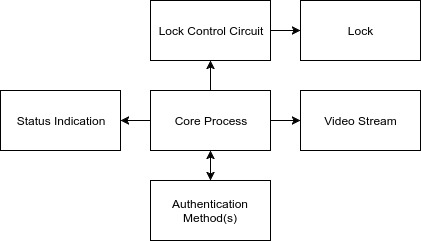
\includegraphics[width=\textwidth]{Diagrams/hardware_block}
    \caption{Hardware Block Diagram}
    \label{fig:hardware-block}
\end{figure}

%---------------------------------------------------------------------------------

\subsection{Lock Control Software Design} \label{lock-control-software-design}

As mentioned in the requirements stated in the previous section, the lock control software should manage the status
LEDs, the lock, and handle incoming authentication data and server interactions. Since the first three elements listed 
are hardware-related operations, creating a layer of abstraction between the between the hardware and the core process 
would increase the cohesion of the design, and prove simpler to implement. This resulted in the first three possible 
classes for the lock control software: one for the abstraction of the LEDs, one for the abstraction of the lock control 
circuit, and one for the abstraction of the hardware interface used for communicating with the authentication modules. 
Since USB is widely used and simple to implement, USB was chosen as the means to connect the modules.

Continuing on with dividing the various responsibilities of the lock control software into subclasses, two more emerge 
from the remaining requirements: one class to poll the authentication modules, which will take advantage of the 
hardware abstraction of the hardware interface, and one class to handle server communication. Figure~\ref
{fig:hardware-block} is a block diagram of the architecture of the lock software.

%---------------------------------------------------------------------------------

\subsection{Authentication Modules} \label{authentication-modules}

To meet the requirement of having a modular framework that supports multiple authentication methods, modules that 
perform the gathering of authentication data can be attached to the system, to increase the authentication options. As 
a result, multiple design patterns emerged immediately in the design of the software for the modules. Interfacing with 
the system core woud be the same across all authentication modules, so only the method used to gather authentication 
data is unique to each module. Two design patterns can be extracted from this statement: an Adapter pattern, where the 
Adaptee provides the interfaces necessary for communicating with the core, and a Template method for handling the 
authentication data. The Adapter can simply implement the Template method, as well as add any other functionality 
necessary for the means of authentication.

With an Adapter pattern in place to handle the creation of various types of authentication modules, there also needed to 
be a pattern to handle the general flow of data, which starts with user entry, and ends with transmission to the system
core. The Entity-Controller-Boundary pattern was a natural fit for this situation, and as shown in 
Figure~\ref{fig:modules-ecb}, the first draft of the authentication module software only required one of each 
stereotype in the pattern, as the software did not need to be complex. The Authenticator object would be passed over 
USB to a controller in the central process.

\begin{figure}
    \includegraphics[width=\textwidth]{Diagrams/modules_ecb}
    \caption{Authentication Modules Pattern Draft}
    \label{fig:modules-ecb}
\end{figure}

In the planning stages of the project, it was intended that the authentication modules would communicate with a central 
single-board microcontroller, such as a Arduino, which would be deemed a "communication board." This communication board
would be responsible for receiving data from the authentication modules, and for error detection and error correction, 
removing that overhead from the central computer. Once all of the authentication data was gathered, the board would send 
the data over a USB connection to the central computer. However, this design was discarded for multiple reasons:
\begin{enumerate}
    \item The Arduino, as well as most other microcontrollers in the hobby market, can only communicate with another 
    Arduino over I2C;
    \item There is only one pair of pins reserved for I2C on most microcontrollers, meaning there can only be one 
    "slave" for each "master" communication board (refer to pinout here);
    \item Connecting all of the authentication modules over USB allowed for far more modularity than the "communication
    board" would have.
\end{enumerate}

Thus, the design changed, in particular to accommodate the final point. Authentication modules would send 
authenticators directly to the core system over USB, with no middle board required. This simplified the design 
considerably, as the behaviour of the authentication modules did not need to change at all, and the responsibilities 
of the communication board were offloaded to the system core. Overall, this design would require fewer 
microcontrollers, while still meeting the requirements.

%=================================================================================

\section{Cloud} \label{cloud}

% TODO: Resolve the comments in my section

\subsection{Amazon Web Servies} \label{amazon-web-servies}

% Double check my reference

Amazon Web Services (AWS) provides a platform to host various cloud services,
including web servers and data storage options~\autocite{AMAZONWEBSERVICES}. In this
project, Amazon Web Services was chosen to host the web server and the database. This
decision was made because the platform is versatile and easy to use, providing a great level of
control where needed but also handling the complicated configuration details automatically.
AWS also provides these services for free within a trial period of one year, making it an even
more attractive choice for a project with limited lifetime. To host the web server, the choice of
programming language and technology, as well as the choice of operating system to run the
server, are left to the user. Similarly, the database technology is a choice of the user, making
AWS a very flexible platform to work with. Amazon Web Services also provides some other
very helpful features, such as domain name services, SSL certificate management, and various
security configuration details to protect the web server and our data. We chose to use AWS
because of the variety of services that were offered that provide everything we needed to
effectively host our web server for this project.

\subsection{Representational State Transer} \label{representational-state-transer}

% Double check my reference
% TODO: Reference the Front Controller section (once written)

The Representational State Transfer (REST) architectural style ~\autocite{RESTARCHSTYLE} was chosen to be used
for our web server. The main principle of REST that we adhered to is the idea of a stateless
server in the client-server relationship. This means that the server does not store any session
information; enough session information must be passed from the client on each request to
identify the necessary information for the request. The benefit of this for the server is that less
information is stored on the server, so less time will be spent contacting the database to
determine session information. Another feature of REST is the idea of a uniform interface. This
helps to keep the system simple by relying on identifiers to specify which resource or service is
needed at the time. The path and the query string in the URL are examples of identifiers that
specify which endpoint or service is being requested. The web server for this project has this
uniform interface as all HTTP requests go to a single Front Controller, which
then determines based on the identifiers the appropriate handler of the request.

\subsection{JavaScript Object Notation} \label{javascript-object-notation}

% Double check my reference (page 7, section 1)

In order to send information between the client and the server, a standard format for
representing the data is necessary. We have chosen to use JavaScript Object Notation (JSON) to
serve this purpose. "JSON is a lightweight, text-based, language-independent data interchange
format" ~\autocite{JSONREF}. JSON provides an easy way of transferring data that is flexible and has support
from many programming languages, making it a very good choice for our project, where
different components will be using different technologies and built in different languages. It is
also very lightweight in terms of its grammar, having very few elements that allow for many
different types of data, keeping the parsing easy which can help to improve response time.

\subsection{Node.js} \label{node.js}

% TODO: Properly reference the AWS section

As mentioned above, Amazon Web Services allows for web
servers written in many languages, leaving the choice of language to the user. In our case we
decided to use Node.js to write our server code. This language was chosen because it is able to
run on multiple operating systems and does not require more than one tool for effective development.
The ability to run on multiple operating systems is very useful to test our code in different ways,
and leaves us with flexibility of which operating system to host the server with. In the early
stages of the project, we considered using C\# with the .NET framework to build the web server,
as some members of the group had experience working with this particular technology in the past
for a similar purpose. After some discussion, it was decided that in order to effectively develop
the application in C\# tools would be needed that are not available on the computers at school,
which would limit our ability to work on the server. This is a major reason that we decided on
Node.js, since it can be very effectively developed using only simple text editors, then can be
executed quickly, without needing to install any build tools. This portability made it very easy to
work on the code in the same development environment whether we were at school or at home.

\subsection{HTML} \label{html}

% TODO: Check if I need to explain HTTP GET request

Hyper Text Markup Language (HTML) is the standard language for creating web pages. HTML describes the
structure and content of a web page through its markup. Web Browsers use an HTML document to render
the content of a web page ~\autocite{HTMLREF}. Since this language is the standard, it was a natural choice for our
project to have the structure and content of the web interface represented in HTML. An HTML document
is returned by the server on an HTTP GET request to the root of the SBACS server URL, and is then
rendered by the client's web browser.

\subsection{JQuery} \label{jquery}

% TODO: Reference the HTML section in this first sentence

The structure and content of the web interface are statically defined using HTML, but this will not
be an interactive web page without the use of JavaScript. JavaScript allows for functionality to be
added to certain actions performed by the user while interacting with the web page. In this project,
we use JavaScript to dynamically modify the content of the web page and retrieve additional
information from the server without requiring a page reload on the client side.

JavaScript has varying levels of support across different web browsers. This introduces a problem as
different clients will have a different user experience, and some functionality may not work for
all clients. JQuery is a library that helps to solve this problem by providing standard functions that
are supported by many different web browsers ~\autocite{JQUERYSUPPORT}. There is also the added benefit
of having functions that
provide more functionality than the default JavaScript functions, making many operations easier on the
programmer. For example, manipulation of the content and structure of the web page is made much simpler through
standard JQuery functions ~\autocite{JQUERYREF}. The support across many browsers and the added functionality make this a
very desirable library to fulfill all of the needs of our web interface.

\subsection{Single Page Application} \label{single-page-application}

% Maybe quote first sentence of the reference?

The web interface is designed to be a Single Page Application (SPA). A Single Page Application is
a web application that runs on a single web page, having no HTML page reloads ~\autocite{SPAREF}. This means
that there is JavaScript performing all requests to the server to retrieve new information, and the
JavaScript is also performing the manipulation of the web page to update the content and structure.
This style of application was chosen in order to keep the server side processing of HTML to a minimum.
Once the page has been returned to the client one time, there will be no more HTML processing on the
server, as all subsequent information is requested through JavaScript. This reduces complexity on the
server processing, as a static HTML file is always returned, and no actual processing of HTML is needed.

\subsection{MySQL} \label{mysql}

To store data that is needed by our system, we decided to use a relational database. All
members of the group have taken at least one course that has talked about relational databases, so
we all had at least some basic understanding of this type of database. MySQL was chosen
because it was known to members of the group, making it easy for everyone to make queries to
the database whenever it was needed.

\subsection{Relational Database Theory} \label{relational-database-theory}

% TODO: explanation of relational theory, third normal form
% TODO: proof of third normal form for our db here
% Database normalization reference: https://www.tutorialspoint.com/sql/sql-rdbms-concepts.htm
We follow third normal form in our database. The proof and description of what that is will go here.

\subsection{Authentication for Server API} \label{authentication-for-server-api}

% TODO: Also include SD for flow of this in detail
% TODO: Maybe?: Mention the hashing algorithm used, maybe explain it

Many requests to the server allow users to read, modify, and delete data, so we needed a
way to ensure that users were identified and authenticated to allow certain requests to be
performed. We used Keyed-Hash Message Authentication Codes (HMAC) to accomplish this goal.
The user is able to login using their username and password, and upon successful login, they are
provided with a key and user id. The key is then used to hash the body of subsequent messages. 
The client must also send the user id to identify who is trying to
make the request. When the server receives the request, it will hash the body of the message as
well using the key that it has stored for that user. If the hashed body that is provided is the same
as what the server gets from hashing the body, then this means that the user is authenticated. The
provided user id is used to determine which key the server will use to hash the message, and is
also used to determine whether or not the user is authorized to make the request they are
attempting to make.

\subsection{Storing Authenticator Data Securely} \label{storing-authenticator-data-securely}

In order to protect user passwords from attacks, the database must not store the
passwords in plain text. If the passwords are in plain text, an attacker could simply read the data
and know the user’s password. To prevent this problem, we use salting, which allows us to store a 
hashed version of the data, along with a salt that is
used to generate the hashed value ~\autocite{PASSWORDSALTING}. To compare a given password by the user to the value that is
stored, the server must retrieve the salt and use it to hash the given password. The hashed value
in the database should then match the hashed given password, meaning that the user has provided
the same password. With this technique, the data is never stored in plain text so it is less
vulnerable to many types of attacks.

\subsection{Sending Data Securely Over the Network} \label{sending-data-securely-over-the-network}

% TODO: Double check that my reference for this is correct, had two authors

The Hypertext Transfer Protocol (HTTP) is the standard protocol used to send requests on the internet ~\autocite{HTTPREF}.
In many situations, these requests need to contain sensitive information, such as passwords or personal
information about the user. Over this HTTP connection, this data cannot be sent securely, as there are
security vulnerabilities in HTTP. In order to send this information securely, HTTPS is the common
solution. In order to ensure the information is sent securely, there is a layer of authentication
and encryption between the client and server for every HTTPS request that is made ~\autocite{HTTPSVSHTTP}. This ensures that
only the sender and intended recipient are able to view and modify the contents of the message. In our
project we have ensured the use of HTTPS wherever it is necessary to protect our sensitive information.


\subsection{Design Patterns} \label{design-patterns}

%TODO: Consider having a higher level section for this, as I think it is important
% TODO: Find GOF book for references about patterns (4806 textbook for Front Controller pattern)

% Patterns to discuss include: Front Controller, MVC, Facade (sign-up), 
% All need a class diagram or similar to prove the pattern is used

Diagrams and descriptions of how certain design patterns were used will go here.


%=================================================================================

% For the physical thing - not sure if this should be here since Michel et al did basically all of this ;)
\section{Lock Demonstration} \label{lock-demonstration}

This chapter will be about the design and construction of the demo unit used at the poster fair

%=================================================================================

\chapter{System Implementation} \label{system-implementation}

This chapter describes the steps taken to implement the SBACS. The tools used along with the design patterns implemented
are described in detail, along with any design decisions that had to be made or changed when the need became apparent.
This chapter also outlines all of the protocols used to facilitate communication between the various devices that make
up SBACS.

%=================================================================================

\section{Android Application Development} \label{android-application-development}

The Android application was developed using Android Studio [] exclusively, and is primarily composed of Java classes, XML
documents, and gradle build files. Android studio was selected since it seemed to be the natural tool for writing an
Android application, and didn't have any negatives with respect to our requirements. Gradle [] was chosen as the build
tool as it is naturally integrated with Android studio.

%---------------------------------------------------------------------------------

\subsection{Server Interfacing} \label{server-interfacing}

Connections to the server were managed through the android Volley API. Volley provides a simple interface over which
HTTP and HTTPS messages can be sent. Standard operation of Volley follows a simple procedure: first a RequestQueue is
set up, and then various Requests are enqueued. These requests are then dequeued by the RequestQueue's thread, which
then creates an HTTP/HTTPS connection. The response that comes back over the connection is handled by another thread.

The code for handling these responses is put in a class that extends a Response.Listener of a given type. The
Response.Listener class provides methods to handle HTTP responses. Since these classes have just a few relatively simple
methods, anonymous classes were used in all cases. Further, we decided that handling the parsing should be done as
safely as possible, so all responses were first parsed simply as Strings. Then, the response was attempted to be parsed
as a JSON object of the type expected from the server. If that parsing failed, the message was instead considered an
error, and handled from there.

%---------------------------------------------------------------------------------

\subsection{HMAC} \label{hmac}

Since the server used HMAC to handle security issues, the application needed to make frequent use of the headers that
the server expected to handle authentication. For this reason, a helper class called HMACHelper, was created. This
class provided methods that were commonly used by all requests about data particular to the current user. Most notably,
HMACHelper provided a method which calculated the secret using the same algorithm that the server would use. To
reiterate how HMAC functions, the body of the message is hashed using a private key shared by the server with the
application. When the application sends data that requires authentication, the server checks that the secret value
provided by the application matches what it calculates using the body of the message as well as the private key
associated with the user. These private keys are generated by the server when the user logs in to the application,
and expire over time, creating the notion of a session.

The precise algorithm used for the hashing function matches the decision made for the server. This is necessary, since
otherwise the secret values would not match between the application and the server. The application relies on a version
of the Password-Based Key Derivation Function algorithm using SHA256 to be available on the Android device. The only
workaround for this added requirement would have been to implement the algorithm (specified in RFC 2898 with test
vectors in RFC 6070) ourselves, however doing so is known to be quite dangerous as any minor error could result in a
security breach. In addition, the number of iterations and the length of the resulting key had to be synchronised
between the server and the application to ensure the values match.

%---------------------------------------------------------------------------------

\subsection{Entity Representation} \label{entity-representation}

The application needed to be able to display data to the user that came from the server and database. These data are
represented in the MVC design of the application. Since the database is relational, the model classes that represent
the constructs stored in the database, such as identities, authenticators, locks, and registrations, were all passive
entity classes whose only real role was to contain data.

Each kind of data that was of interest to the user was given its own Activity, which is similar to the notion of a page
in a web application. These Activities were all primarily composed of a ListView object, which displays a list of data.
This list was configured with an Adapter class which extends the general ArrayAdapter<T> class. These adapters were
used to convert the model classes into a view. The adapter classes were composed of an XML file which described the
layout of the view, as well as a Java class which provided the methods by which the data could be used to fill in the
layout.

%=================================================================================

\section{Hardware} \label{hardware}

The hardware portion of the project consisted of three components: the lock control circuit, the lock control software, 
and the authentication modules.

\subsection{Lock Control Circuit Implementation} \label{section:lock-control-circuit-implementation}

Since driving the LEDs and the electrical lock only requires digital output, no analog pins would be necessary. While 
the single-board microcontrollers considered had optional boards which could add Wifi or Ethernet capabilities, they 
would not have been a sufficient solution to run the core process, as they were lacking a sufficient number of USB 
ports, and the overhead for implementing the core would have been too high. Because the microcontrollers do not run an 
operating system, 

A Raspberry Pi was ultimately selected as the computer to run the core process. The Pi 3 Model B has four USB ports, 
built-in Wifi capability, and forty pins for general-purpose IO (GPIO). These hardware features made the Raspberry Pi the best 
out-of-the-box solution to run the core process.

\subsection{Lock Control Circuit} \label{lock-control-circuit}

The next design problem to consider was the means to control the status of the electric lock. The simplest locks 
available, solenoid locks and electric strike locks, do not include any control mechanisms. They are either powered on, 
to disengage the lock, or powered off and locked. Therefore, it was necessary to implement a circuit to control the power to the 
lock, with the switching being driven by one of the Raspberry Pi's GPIO pins. There were two options considered for 
this:

1- Transistor/diode circuit

This circuit would use a TIP120 Darlington transistor, coupled with a 1N4004 flyback diode, to drive the lock. This 
circuit is demonstrated in figure X.

Todo: Make the figure of the transistor/diode circuit in Fritzing

The major issue with this circuit is that 

Some heat-related math for the transistor:
The power law for a single voltage drop is $ P = IV = I^2R $. A transistor can be treated as two voltage drops, one 
from base to emitter ($ V_{BE} $), and another from collector to emitter ($ V_{CE} $), resulting in the power dissipated
by a transistor being given by:
$$ P = V_{BE}I_B + V_{CE}I_C $$
Since $ I_B \ll I_C $ when the lock circuit is active, the $ V_{BE}I_B $ term is negligible in this case, so the power
dissipated by the transistor is given by:
$$ P = V_{CE}I_C $$
At steady state, the voltage drop from the solenoid is negligible, as $ \frac{di}{dt} $ is zero, resulting in $ V = 
L\frac{di}{dt} = 0 $. This means that the voltage drop across the transistor, from emitter to collector, is 12V. Given
that the solenoid draws $\SI{650}{\milli\ampere}$ of current, the power across the transistor is:
$$ P = \SI{12}{\volt} \times \SI{650}{\milli\ampere} $$
$$ P = \SI{7.8}{\watt} $$
This power dissipation is quite significant in comparison to, for example, the resistors in the LED circuit, which at 
most will dissipate about $\SI{50}{\milli\watt}$. (n.b. should I put the math behind this in an appendix?) A heat 
dissipation mechanism would be necessary to ensure that the system does not heat up dangerously while in operation, 
which may not be practical in a real-life scenario. Secure systems should be completely enclosed, as a fan would 
introduce a point of physical access to the system.

Insert some more math and talk about the flyback diode to deal with the voltage spike - take the lock to a DOE lab at 
some point and measure the voltage spike when 12V DC is applied, to see what the minimum RB breakdown voltage should be

2- Relay circuit

Internally, a relay is very similar to the transistor/diode circuit, with a mechanical switch added. The relay itself 
has three inputs, and three outputs. The inputs are a positive voltage ($ V_{CC} $), ground (GND), and an input signal 
(IN). The outputs are a normally-closed terminal (NC), a common terminal (CO), and a normally-open terminal (NO). The 
circuit diagram of a relay is shown in Figure~\ref{fig:relay-circuit-diagram}.

\begin{figure}
    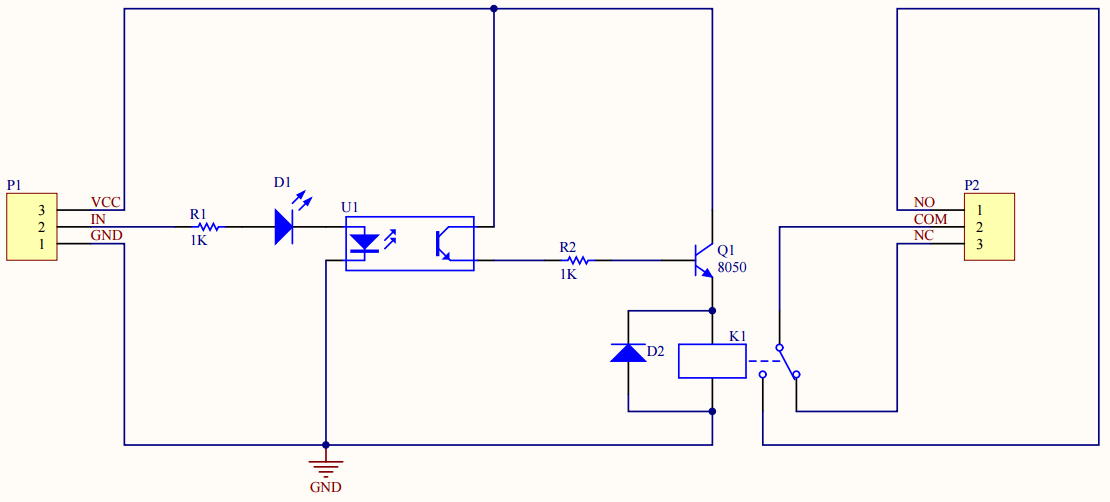
\includegraphics[width=\textwidth]{Diagrams/relay_circuit}
    \caption{Relay Circuit Diagram~\autocite{RELAYCIRCUIT}}
    \label{fig:relay-circuit-diagram}
\end{figure}

What separates the relay from a transistor/diode circuit is that it uses a solenoid internally to flip a mechanical 
switch. When the IN signal is low (0 volts), the switch short-circuits the "normally closed" connection, allowing
current to flow from the NC terminal to the CO terminal. The NO terminal is open-circuited, so no current will flow.
When the IN signal is high (5 volts), the solenoid inside the relay generates a magnetic field, which causes the switch 
to instead short-circuit the "normally open" connection, allowing current to flow from the NO terminal to the CO 
terminal, while the NC terminal is open-circuited. 

The final layout for the lock control circuit is demonstrated in figure ~\ref{fig:lock-control-circuit-diagram}.

\begin{figure}
    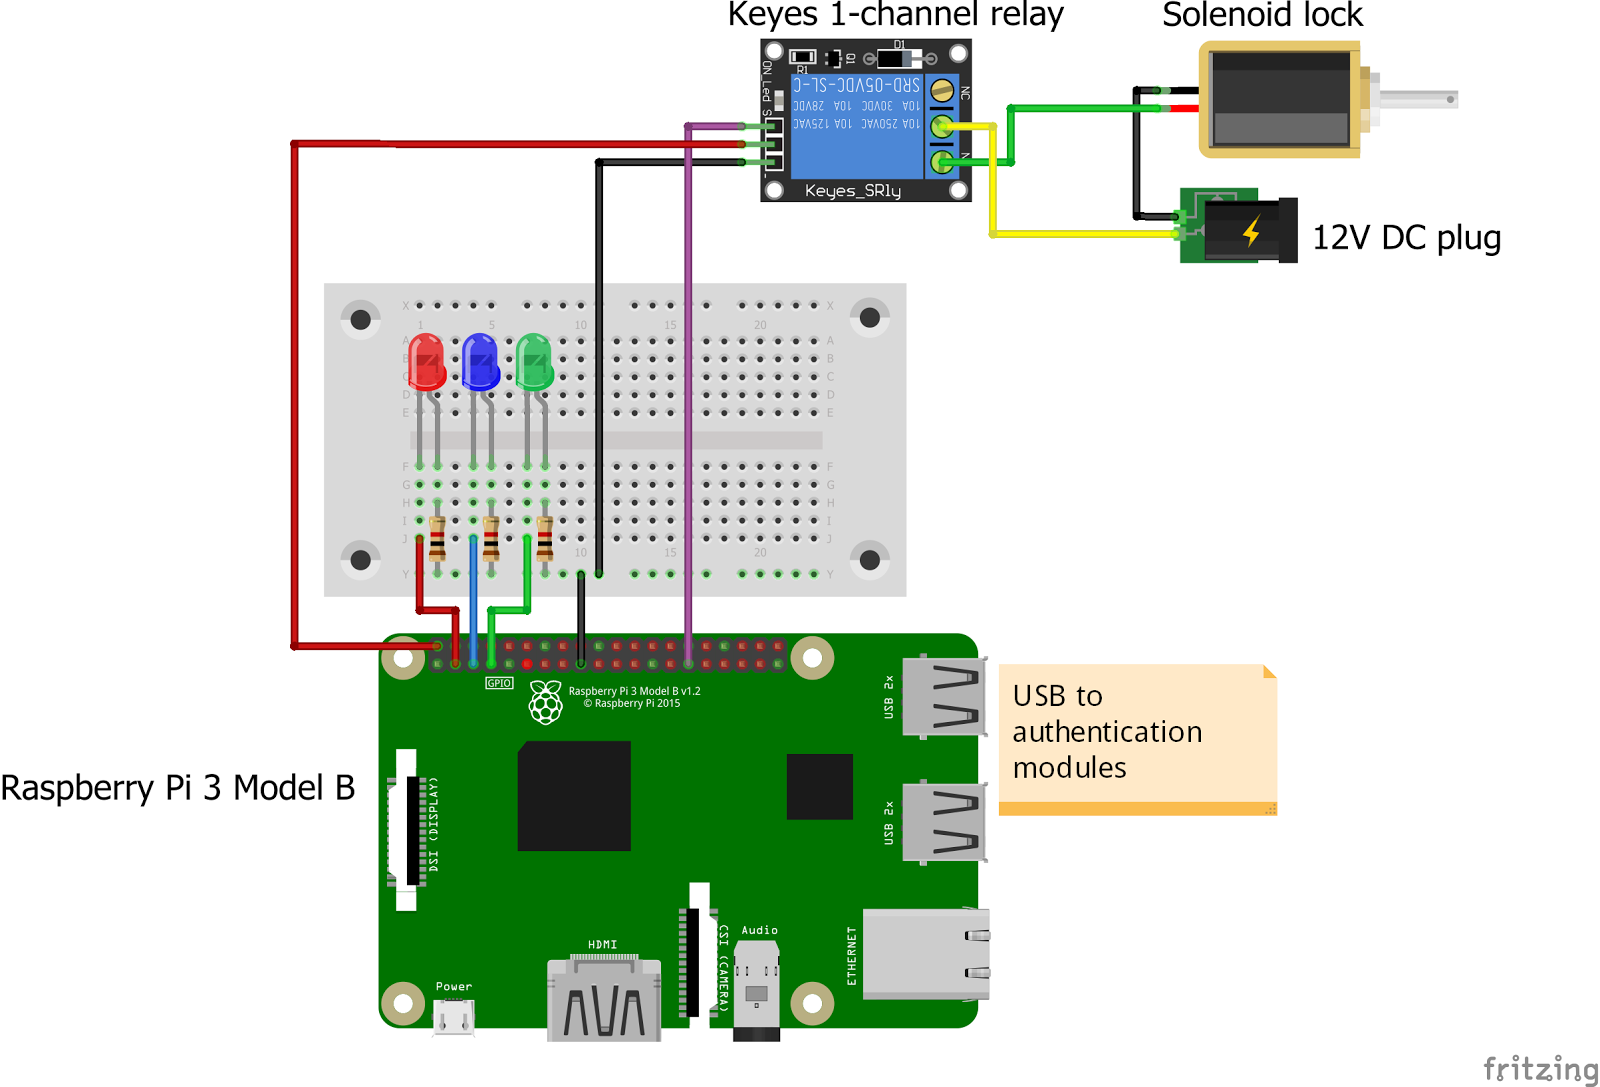
\includegraphics[width=\textwidth]{Diagrams/hardware_lock_control}
    \caption{Lock Control Circuit}
    \label{fig:lock-control-circuit-diagram}
\end{figure}

\subsection{Lock Control Software} \label{lock-control-software}

% To realize the design outlined in section

\subsection{Authentication Module Implementations} \label{authentication-modules-implementations}

\subsubsection{NFC Module} \label{nfc-modules}

\subsubsection{PIN Module} \label{pin-modules}

%=================================================================================

\section{Cloud Sewrvices} \label{cloud-services}

%TODO: Talk about node http library, crypto library, url library, mysql library

%TODO: Generally developed using Notepad++, Postman to test it

% My problems/solutions section
% TODO: Reference relevant sections of earlier part throughout this section (AWS, HTTPS, Database stuff)
\subsection{Learning to Use Amazon Web Services} \label{learning-to-use-amazon-web-services}

Amazon Web Services provides all the hosting that we needed for this project, so it was a
natural choice for us to use. When we started, we followed some basic tutorials to get a sample
web application running, that would return a static HTML page on all HTTP requests. The first
major challenge came from attempting to modify this sample application. First, we had to find
the code of the sample application, as it was not given in any location that we thought to look on
AWS. Eventually we found the code and modified it, then building and testing it locally to
ensure that the code was correct. Then we had to deploy this new code, which proved to be
harder than expected. The process is not complicated once it is known, but the wording was
confusing in the instructions, so it took a few tries to get it working. Once we had this process
figured out, we were able to easily write our own code and the process of updating our hosted
server was easy.

The next challenge in learning AWS came from the database. Since we needed a
persistent data storage, and had decided on a relational database, we decided to set up our
database using AWS as well, which allowed us to keep all hosted services in one place. Initially,
we created the database from the management console of our hosted web application. This made
it easy to get a database setup and working with our server in very little time, but we soon
realized that it was tied to the web application, and could not exist without the web application.
This was not ideal, since the database should be able to exist separately, so we ended up deleting
that database, and hosting one from the relational database manager on AWS. This kept it
completely separate from the server, but still usable by the server. Another challenge was
introduced when we tried to access the database directly, to initially build the tables and data,
and to have the ability to query it later on. We were not all able to access the database, and we
were unsure why, since we all were using the same tools, with the same settings to do it.
Eventually we discovered that the database itself has settings to allow certain IP addresses to
access it directly. We all agreed that this was a very smart feature, but we simply did not realize
it existed at first. Once we discovered this, we were able to add the IP addresses of our
computers as we needed to, but left the general public unable to access our database, keeping it
secure.

We also had to learn more about how AWS handles SSL certificates and domain names,
so that we could use HTTPS instead of HTTP to transfer user information securely. We realized
we would need a domain name for certain features of our system, so we used AWS to purchase
our domain name, and then to route requests to that domain name to our hosted server. This was
not very complicated, but still had some learning to get it done correctly, and involved some
change to configuration files on our server that we did not know existed up to that point. The
specific troubles with SSL Certificates will be explained in more detail in the following section.

\subsection{SSL Certificates} \label{ssl-certificates}

%TODO: Reference section in 5.5 about HTTPS and SSL stuff

In order to send requests over HTTPS instead of HTTP, SSL Certificates are needed.
These provide an extra layer of security to ensure that only the sending and receiving parties are
aware of the content of the message.
SSL Certificates were a challenge to understand and work with, as none of us had much
knowledge about them before. Certificates must be signed in order for them to be considered
valid. This signing can be done by a developer, but the certificate must be explicitly declared as
valid on each device that will have contact with the server over HTTPS in this case. This would
be very hard to manage and is not practical for an application with many users. In order for most
devices to know by default that it should be accepted, the certificates must be signed by a
Certificate Authority. The Certificate Authorities are known to browsers and let the devices know
that the destination can be trusted.

For our project it was decided that it would be easier for everyone if the certificates were
signed by a Certificate Authority, to keep things simple. Unfortunately, this process can take
time to get approved, and there is still some configuration to be managed by the server to work
correctly. AWS handles many of these complications, and also handles the generation and
signing of the certificates, but in order to do this, a domain name must be owned. Using AWS for
this was the best option we found for this problem, so we bought a domain name, and we were
able to get the SSL Certificates, and had HTTPS working quickly after that.


\subsection{Issues with String Encodings} \label{issues-with-string-encodings}
% More than just server issue, but problem was on server

When the database was first built, we decided to store authentication data as strings. This
was chosen because we found strings easy to work with, and most HTTP libraries had support
for sending data as strings. During the integration phase of the project, we started having trouble
with authentication, where the data that was retrieved from the server by the phone was then sent
to the lock controller and then sent back to the server for validation. The server was receiving
different data than it was initially sending, so all requests to unlock were being denied. After
debugging at different points in the system, we came to the conclusion that the encoding of
strings was not the same across the languages and technologies we were using, so the data was
not the same when it reached the server again.

To solve this problem, we changed the data types stored by the database to be binary data
rather than strings. This eliminated the problem of encoding, since binary data is simply binary
regardless of the platform or technology being used. We realized that it would have made more
sense to go with a binary data type in the beginning, but we did not anticipate the problems with
encoding initially. This problem took a long time to identify, and was the largest delay in our
integration phase of the project.


\subsection{Improving Response Time} \label{improving-response-time}

The system needs to respond quickly to inputs from the user in order to provide the best
user experience. One limiting factor of this response time is the communication with the cloud
server. Sending a request over the network is very slow relative to other actions in the system, so
the response from the server must be as quick as possible to minimize the delay. In order to keep
this fast, the main goal of the server is to have a response sent as early as possible to the user.
Many actions are dependent on one another, but in a few cases the response can be sent to the
user before all the actions associated with the request have actually finished. For example, when
a user logs in, the server must check that they have provided sufficient authentication to be
logged in. Once this has been validated, the user is considered to be logged in. At this point, the
server sends a key to the user that is valid for a limited time, which is used by the Android
application to provide NFC authentication, and is also used in the authentication on subsequent
requests to the server. After this key is sent back to the user, the server must still save this key if
it is newly created, and must save the key as the NFC authenticator for the user. Since these
actions can happen after the key is sent, the response will be returned faster.

Another limiting factor in the speed of server response is contact with the database. This
can be slow, as the database may have a large amount of information to go through. To solve this
problem, the server sends as few queries as possible, that will collect all the information that is
needed for the request, but will not retrieve data that is unnecessary. Less queries to the database
keeps the delay in sending and receiving responses low, allowing the server to spend less time
waiting and more time processing information.



%=================================================================================

\chapter{Testing and Bug Fixes} \label{testing-and-bug-fixes}

% Not really sure what to go with here
Points to mention in this chapter:
\begin{itemize}
    \item Our biggest bug - issues with sending bytes "in the raw" using JSON
    \item Limitation on the number of bytes in NFC data exchanges using the PN532 shield
    \item The many struggles of serial communication (e.g. the Serial Monitor in the Arduino IDE, certain input flags 
    on a port would be enabled by default on some machines but not others)
\end{itemize}

\section{Bugs} \label{bugs}

\subsection{Issues with Serial Communication} \label{issues-with-serial-communcation}

%=================================================================================

\chapter{Conclusions} \label{conclusions}

%=================================================================================   

\addcontentsline{toc}{chapter}{Bibliography} % Need this so it appears in the ToC
\printbibliography

%=================================================================================

\appendix

%=================================================================================

\chapter{Sample Appendix} \label{sample-appendix}



\end{document}

